\documentclass[a4paper]{article}

\usepackage{amsmath}
\usepackage{amsfonts}
\usepackage{tikz}

\title{A fixed point semantic for FIRRTL programs}
\author{David N. Jansen, Keyin Wang, Xiaomu Shi\thanks{Institute of Software, Chinese Academy of Sciences, Beijing, China}}

\newcommand{\portsem}{\mathsf{PortSumm}}
\newcommand{\stmtsem}{\mathsf{StmtSumm}}
\newcommand{\expressions}{\mathsf{exprs}}
\newcommand{\flippedexpressions}{\mathsf{FLIPPEDexprs}}
\newcommand{\emptylist}{[\,]}
\newcommand{\rconslist}[2]{[#1 \mathbin{::} #2]}
\newcommand{\concatlist}[2]{#1 \mathrel{++} #2}
\newcommand{\needtobedefined}{\text{\textsf{to-be-defined}}}
\newcommand{\undefinedonpurpose}{\text{\textsf{undefined-on-purpose}}}
\newcommand{\extractinput}[2]{\mathsf{inp}_{#2}(#1)}

\begin{document}

\maketitle

\section{Introduction}

FIRRTL is an intermediary language to describe hardware circuits.
It allows some variation, from HiFIRRTL including a few higher-level constructs, e.g. case distinctions through “when” statements and aggregate data types, to LoFIRRTL, which can almost directly be mapped to a netlist.

While there are existing LoFIRRTL semantics, more or less formal ones, the official documentation only provides an informal, textual description of the HiFIRRTL semantics.
The reference implementation provides a kind of formal semantics through a translation from HiFIRRTL to LoFIRRTL.
In discussions within our FIRRTL verified compiler working group, we formed several ideas for mathematically sound HiFIRRTL semantics.

One difficulty with HiFIRRTL semantics is an allowed form of underspecification:
in a module, one does not need to indicate all signal widths;
the compiler is then supposed to find the smallest signal width that will not lead to data loss.
Also, it is allowed to leave undetermined whether a reset wire shall be synchronous (i.e.\@ resets will happen only at a rising clock edge) or asynchronous (i.e.\@ resets will happen immediately when the reset wire gets high).
When underspecified components are connected with fully specified ones, the underspecification is resolved.
It is an error if components with inconsistent reset types are connected.
This also shows that it is difficult to make the semantics fully compositional:
some parts of the semantics are determined by the context of a component.

We earlier tried to define a semantics along the following lines: underspecified components do not get a single semantic interpretation, but a set of possibilities.
During the InferWidths pass of the compiler, the widths are then determined, leading to a circuit with a unique semantic interpretation, which is the possibility with the smallest signal widths.

In this note, I want to propose another semantic, based on an idea brought into the discussion by Yicheng Liu (?).
The basic idea is to create a connection summary, that is a function describing all combinatorial connections in the module,
and then iterate this function until a fixed point is reached.
If no fixed point exists, the module is erroneous.

\textbf{TODO:} Perhaps the semantics of a circuit can be constructed similarly, as the fixed point of the mutual application of all the connection summaries of modules? \textbf{:END TODO}

\section{Connection summaries}

A \emph{FIRRTL circuit} consists of a set of modules, together with an indication which module is the main module.
(Intuitively, the main module is instantiated, and whatever the main module requires as submodules is instantiated as well.)

A \emph{FIRRTL module} consists of a list of ports (describing the interface of the module) and a list of statements (describing the internal connections, registers, submodules etc.\@ of the module).

A \emph{port} has a name, a direction (``input'' or ``output'') and a type.
In HiFIRRTL, the type may be aggregate (a vector/array or a bundle/record type), and its numeric ground components may have underspecified widths or abstract reset types.

From a FIRRTL module, we construct a \emph{connection summary.}
The connection summary is a function that maps the (input connectors of) components in the module to formal expressions constructed from the (output connectors and flipped input connectors of) components.
A second function maps the flipped output connectors of components in the module to formal expressions constructed in the same way.
In these functions, values assigned to read-only parts will just be ignored
(this simplifies the definition if one assigns an aggregate value to a component).

For every component, we also need its kind and data type.
(From the kind one can derive the flow orientation, in particular whether the component is writable.)
The connection summary then has type $C \to \mathit{kind} \times \mathit{datatype} \times \expressions(C) \times \expressions(C)$.
$\mathit{kind} = \{ \mathtt{Inport}, \mathtt{Outport}, \mathtt{Wire}, \mathtt{Register}, \mathtt{Node} \}$ indicates the kind of component.
(Later we might extend this with instance and memory.)
$\mathit{datatype}$ just indicates the data type (signed/unsigned integer and its width, clock, reset signal, array or bundle).
%$\mathit{orient} = \{ \mathtt{Source}, \mathtt{Sink}, \mathtt{Duplex}, \mathtt{Passive} \}$ indicates the orientation/flow direction of the component.
%Perhaps, instead of orientation, we will need the kind (input port, output port, node, wire, register, [memory,] instance).

We now define the connection summary recursively.
Assume given a FIRRTL module $(\mathit{name}, \mathit{portlist}, \mathit{stmtlist})$.
We first construct the connection summary of the port list:
\begin{description}
\item[Empty port list:]
        $\portsem(\mathit{name}, \linebreak[0] \emptylist)$ is the empty function $f : \emptyset \to \mathit{kind} \times \mathit{datatype} \times \expressions(\emptyset) \times \expressions(\emptyset)$.

\item[Input port:]
	If $\portsem(\mathit{name}, \linebreak[0] \mathit{portlist}) = f: C \to \mathit{kind} \times \mathit{datatype} \times \expressions(C) \times \expressions(C)$
	and $\mathit{ip} \notin C$,
	then $\portsem(\mathit{name}, \linebreak[0] \rconslist{\mathit{portlist}}{\mathtt{input~} \mathit{ip} : t}) = f': C \cup \{ \mathit{ip} \} \to \mathit{kind} \times \mathit{datatype} \times \expressions(C \cup \{ \mathit{ip} \}) \times \expressions(C \cup \{ \mathit{ip} \})$,
	defined by $f'(c) = f(c)$ for all $c \in C$ and $f'(\mathit{ip}) = (\mathtt{Inport}, t, \linebreak[0] \needtobedefined, \linebreak[0] \needtobedefined)$.

\item[Output port:]
	If $\portsem(\mathit{name}, \linebreak[0] \mathit{portlist}) = f: C \to \mathit{kind} \times \mathit{datatype} \times \expressions(C) \times \expressions(C)$
	and $\mathit{op} \notin C$,
	then $\portsem(\mathit{name}, \linebreak[0] \rconslist{\mathit{portlist}}{\mathtt{output~} \mathit{op} : t}) = (f': C \cup \{ \mathit{op} \} \to \mathit{kind} \times \mathit{datatype} \times \expressions(C \cup \{ \mathit{op} \}) \times \expressions(C \cup \{ \mathit{op} \})$,
	defined by $f'(c) = f(c)$ for all $c \in C$ and $f'(\mathit{op}) = (\mathtt{Outport}, t, \linebreak[0] \needtobedefined, \linebreak[0] \needtobedefined)$.

	(Note the asymmetry: output ports are defined to be duplex, while input ports are defined to be sources.)
\end{description}
Then we define the (combinatorial) connection summary of the statement list.
One of the inputs is $f_\mathrm{port}$, the function normally generated by the port list (but occasionally a different function).
\begin{description}
\item[Empty statement list:]
	$\stmtsem(\mathit{name}, \linebreak[0] f_\mathrm{port}, \linebreak[0] \emptylist) = f_\mathrm{port}$.

\item[Wire definition:]
	If $\stmtsem(\mathit{name}, \linebreak[0] f_\mathrm{port}, \linebreak[0] \mathit{stmtlist}) = f: C \to \mathit{kind} \times \mathit{datatype} \times \expressions(C) \times \expressions(C)$
	and $\mathit{wr} \notin C$,
	then $\stmtsem(\mathit{name}, \linebreak[0] f_\mathrm{port}, \linebreak[0] \rconslist{\mathit{stmtlist}}{\linebreak[0] \mathtt{wire~} \mathit{wr} : t}) = f': C \cup \{ \mathit{wr} \} \to \mathit{kind} \times \mathit{datatype} \times \expressions(C \cup \{ \mathit{wr} \}) \times \expressions(C \cup \{ \mathit{wr} \})$,
	defined by $f'(c) = f(c)$ for all $c \in C$ and $f'(\mathit{wr}) = (\mathtt{Wire}, t, \linebreak[0] \needtobedefined, \linebreak[0] \needtobedefined)$.

\item[Register definition:]
	If $\stmtsem(\mathit{name}, \linebreak[0] f_\mathrm{port}, \linebreak[0] \mathit{stmtlist}) = f: C \to \mathit{kind} \times \mathit{datatype} \times \expressions(C) \times \expressions(C)$
	and $\mathit{rg} \notin C$,
	then $\stmtsem(\mathit{name}, \linebreak[0] f_\mathrm{port}, \linebreak[0] \rconslist{\mathit{stmtlist}}{\linebreak[0] \mathtt{reg~} \mathit{rg} : t}) = f': C \cup \{ \mathit{rg} \} \to \mathit{kind} \times \mathit{datatype} \times \expressions(C \cup \{ \mathit{rg} \}) \times \expressions(C \cup \{ \mathit{rg} \})$,
	defined by $f'(c) = f(c)$ for all $c \in C$ and $f'(\mathit{rg}) = (\mathtt{Register}, t, \mathit{rg}, \undefinedonpurpose)$.
	(Because the type of a register must be passive, no connection will really change the last component of $f'(\mathit{rg})$.)

	\textbf{TODO:} There may be an additional connection in $f'$ to express the reset. \textbf{:END TODO}

\item[Node definition:]
	If $\stmtsem(\mathit{name}, \linebreak[0] f_\mathrm{port}, \linebreak[0] \mathit{stmtlist}) = f: C \to \mathit{kind} \times \mathit{datatype} \times \expressions(C) \times \expressions(C)$
	and $\mathit{nd} \notin C$ and $\mathit{expr} \in \expressions(C) \setminus \{ \needtobedefined, \linebreak[0] \undefinedonpurpose \}$,
	then $\stmtsem(\mathit{name}, \linebreak[0] f_\mathrm{port}, \linebreak[0] \rconslist{\mathit{stmtlist}}{\linebreak[0] \mathtt{node~} \mathit{nd} = \mathit{expr}}) = f': C \cup \{ \mathit{nd} \} \to \mathit{kind} \times \mathit{datatype} \times \expressions(C \cup \{ \mathit{nd} \}) \times \expressions(C \cup \{ \mathit{nd} \})$,
	defined by $f'(c) = f(c)$ for all $c \in C$ and $f'(\mathit{nd}) = (\mathtt{Node}, \mathit{type}(\mathit{expr}), \linebreak[0] \mathit{expr}, \linebreak[0] \undefinedonpurpose)$.

\item[Unidirectional connect statement:]
	If $\stmtsem(\mathit{name}, \linebreak[0] f_\mathrm{port}, \linebreak[0] \mathit{stmtlist}) = f: C \to \mathit{kind} \times \mathit{datatype} \times \expressions(C) \times \expressions(C)$
	and $\mathit{ref}$ is a writable reference derived from $C$ and $\mathit{expr} \in \expressions(C) \setminus \{ \needtobedefined, \linebreak[0] \undefinedonpurpose \}$ of compatible, passive types,
	then $\stmtsem(\mathit{name}, \linebreak[0] f_\mathrm{port}, \linebreak[0] \rconslist{\mathit{stmtlist}}{\linebreak[0] \mathtt{connect~} \mathit{ref}, \linebreak[0] \mathit{expr}}) = f': C \to \mathit{kind} \times \mathit{datatype} \times \expressions(C) \times \expressions(C)$,
	defined by:
	Let $b = \mathit{base}(\mathit{ref})$.
	If $\mathit{subfield}(\mathit{ref})$ is an unflipped part of $b$, then $f'(b) = (f_1(b), \linebreak[0] f_2(b), \linebreak[0] [f_3(b) \mathrel{\textsc{except}} \mathord{!}\mathit{subfield}(\mathit{ref}) = \mathit{expr}], f_4(b))$.
	If $\mathit{subfield}(\mathit{ref})$ is a    flipped part of $b$, then $f'(b) = (f_1(b), \linebreak[0] f_2(b), \linebreak[0] f_3(b), \linebreak[0] [f_4(b) \mathrel{\textsc{except}} \mathord{!}\mathit{subfield}(\mathit{ref}) = \mathit{expr}])$.
	Further $f'(c) = f(c)$ for all $c \in C \setminus \{ b \}$.

	Here, $\mathit{base}(\mathit{ref})$ is the base identifier of the reference $\mathit{ref}$.
	The \textsc{except} clause indicates that the sub-component indicated in $\mathit{ref}$ is set to the new value
	(and the rest remains the same).
	These functions can be defined recursively
	(they are partial functions because they require type compatibility).

	It would be sufficient to change both $f_3$ and $f_4$ always, because $\mathit{expr}$ must have a passive type,
	and then the other part would be just ignored.

% hfexpr and href are mutually recursive

%What is an aggregate expression? (always there is the requirement of type compatibility)
%Gexpr : fgtyp -> hfexpr -> aggregate_expression
%Aexpr : array_expr -> aggregate_expression
%Bexpr : bundle_expr -> aggregate_expression
%to_be_defined : ftype -> aggregate_expression
%undefined_on_purpose : ftype -> aggregate_expression

%array_expr : seq aggregate_expression -> array_expr

%bundle_expr : name -> aggregate_expression -> bundle_expr -> bundle_expr
%bundle_expr_flipped : name -> faggregate_expression -> bundle_expr -> bundle_expr
%empty_bundle_expr : bundle_expr

%To provide for flipped fields, we should have everything in a flipped variant as well...

%fGexpr : fgtyp -> faggregate_expression (* only determine the type, do not really assign a value *)
%fAexpr : farray_expr -> faggregate_expression (* only assign to flipped parts of the array *)
%fBexpr : fbundle_expr -> faggregate_expression

%farray_expr : ftype -> seq faggregate_expression -> farray_expr

%fbundle_expr : name -> ftype -> faggregate_expression -> fbundle_expr -> fbundle_expr
%fbundle_expr_flipped : name -> ftype -> aggregate_expression -> fbundle_expr -> fbundle_expr
%fempty_bundle_expr : fbundle_expr

%The type of an aggregate expression can be constructed from its structure and the types of the ground expressions.
%The aggregate expressions in an array expression should all have the same / compatible types.
%(Compatibility is tested similarly to multiplexer types.)
%In bundle expressions, field names should be unique.
%If the aggregate expression is not well-formed, its type is None.

%-----

%Then an assignment is a (partial) function from names to aggregate expressions.
%Actually two functions: also a partial function from names to faggregate expressions.
%(Non-passive) duplex and source values are defined in the second function;
%Duplex and sink values are defined in the first function.
%The types of the expressions of duplex components must be compatible.

%(Registers are duplex but passive, so one does not actually need to assign an faggregate expression, as it must always be empty.)
%Curiously, output ports are duplex (not sinks) and input ports are sources---not sure where this difference comes from. Perhaps because sometimes one wants to read from the output port?

%Then a connect statement updates these functions.
%The update can be defined recursively by a function
%update_value : aggregate_expression (*old value*) -> href (*reference to the part that is updated*) -> aggregate_expression (*new value*) -> option aggregate_expression
%fupdate_value : faggregate_expression etc.
%
%If href is a simple reference, the result is the new value (if the two types are compatible; otherwise it is None).
%Flipped parts are not changed because flipped expressions do not contain a value!
%If href is an array access, then the old value must be an array expression, and the update is composed from the old value and update_value of the one array element that was accessed
%If href is a bundle access, then the old value must be a bundle expression, and the update is composed from the old value and update_value of the one field that was accessed.
%If the field was flipped, then the update should go the other way--not sure how to implement that.

%A bidirectional connect statement updates two values in the function. Perhaps we can have a flipped update function, which updates the flipped parts?
%(Perhaps build this into the normal connect function with a boolean switch whether it's a flipped update or not.)

\item[Bidirectional connect statement:]
	If $\stmtsem(\mathit{name}, \linebreak[0] f_\mathrm{port}, \linebreak[0] \mathit{stmtlist}) = f: C \to \mathit{kind} \times \mathit{datatype} \times \expressions(C) \times \expressions(C)$
	and given writable references $\mathit{ref}_1$ and $\mathit{ref}_2$ derived from $C$ of compatible (not necessarily passive) types,
	then $\stmtsem(\mathit{name}, \linebreak[0] f_\mathrm{port}, \linebreak[0] \rconslist{\mathit{stmtlist}}{\linebreak[0] \mathtt{connect~} \mathit{ref}_1, \linebreak[0] \mathit{ref}_2}) = f': C \to \mathit{kind} \times \mathit{datatype} \times \expressions(C) \times \expressions(C)$,
	defined by:
	Let $b_1 = \mathit{base}(\mathit{ref}_1)$ and $b_2 = \mathit{base}(\mathit{ref}_2)$.
	If $\mathit{subfield}(\mathit{ref}_1)$ is an unflipped part of $b_1$, then $f'(b_1) = (f_1(b_1), \linebreak[0] f_2(b_1), \linebreak[0] [f_3(b_1) \mathrel{\textsc{except}} \mathord{!}\mathit{subfield}(\mathit{ref}_1) = \mathit{ref}_2], f_4(b_1))$.
	If $\mathit{subfield}(\mathit{ref}_1)$ is a    flipped part of $b_1$, then $f'(b_1) = (f_1(b_1), \linebreak[0] f_2(b_1), \linebreak[0] f_3(b_1), \linebreak[0] [f_4(b_1) \mathrel{\textsc{except}} \mathord{!}\mathit{subfield}(\mathit{ref}_1) = \mathit{ref}_2])$.%
	---If $\mathit{subfield}(\mathit{ref}_2)$ is a    flipped part of $b_2$, then $f'(b_2) = (f_1(b_2), \linebreak[0] f_2(b_2), \linebreak[0] [f_3(b_2) \mathrel{\textsc{except}} \mathord{!}\mathit{subfield}(\mathit{ref}_2) = \mathit{ref}_1], f_4(b_2))$.
	If $\mathit{subfield}(\mathit{ref}_2)$ is an unflipped part of $b_2$, then $f'(b_2) = (f_1(b_2), \linebreak[0] f_2(b_2), \linebreak[0] f_3(b_2), \linebreak[0] [f_4(b_2) \mathrel{\textsc{except}} \mathord{!}\mathit{subfield}(\mathit{ref}_2) = \mathit{ref}_1])$.
	Further $f'(c) = f(c)$ for all $c \in C \setminus \{ b_1, b_2 \}$.

\item[When statement:]
	If $\stmtsem(\mathit{name}, \linebreak[0] f_\mathrm{port}, \linebreak[0] \mathit{stmtlist}) = f: C \to \mathit{kind} \times \mathit{datatype} \times \expressions(C) \times \expressions(C)$
	and given $\mathit{cond} \in \expressions(C)$, and statement lists $\mathit{truestmtlist}$ and $\mathit{falsestmtlist}$,
	then $f' := \stmtsem(\mathit{name}, \linebreak[0] f_\mathrm{port}, \linebreak[0] \rconslist{\mathit{stmtlist}}{\linebreak[0] \mathtt{when~} \mathit{cond} \linebreak[0] \mathtt{~then~} \mathit{truestmtlist} \linebreak[0] \mathtt{~else~} \mathit{falsestmtlist}})$ is defined as follows.

	Let $f_\mathrm{true} : C_\mathrm{true} \to \mathit{kind} \times \mathit{datatype} \times \expressions(C_\mathrm{true}) \times \expressions(C_\mathrm{true}) := \stmtsem(\mathit{name}, \linebreak[0] f, \linebreak[0] \mathit{truestmtlist})$ and
	$f_\mathrm{false} : C_\mathrm{false} \to \mathit{kind} \times \mathit{datatype} \times \expressions(C_\mathrm{false}) \times \expressions(C_\mathrm{false}) := \stmtsem(\mathit{name}, \linebreak[0] f, \linebreak[0] \mathit{falsestmtlist})$.
	(Note that we do not use $f_\mathrm{port}$ but $f$ here.)

	We define $f' : C_\mathrm{true} \cup C_\mathrm{false} \to \mathit{kind} \times \mathit{datatype} \times \expressions(C_\mathrm{true} \cup C_\mathrm{false}) \times \expressions(C_\mathrm{true} \cup C_\mathrm{false})$ to be:
	\begin{itemize}
	\item	If $(C_\mathrm{true} \setminus C) \cap (C_\mathrm{false} \setminus C) \not= \emptyset$, there is an error.
	\item	For $c \in C_\mathrm{true} \setminus C$, we have $f'(c) = f_\mathrm{true}(c)$.
	\item	For $c \in C_\mathrm{false} \setminus C$, we have $f'(c) = f_\mathrm{false}(c)$.
	\item	For $c \in C$, we have $f'(c) = (f_1(c), \linebreak[0] f_2(c), \linebreak[0] \mathsf{mux}(\mathit{cond}, f_{\mathrm{true},3}(c), f_{\mathrm{false},3}(c)), \linebreak[0] \mathsf{mux}(\mathit{cond}, f_{\mathrm{true},4}(c), f_{\mathrm{false},4}(c)))$.
	\end{itemize}
	\textbf{TODO:} If a component is defined only in $\mathit{truestmtlist}$ or in $\mathit{falsestmtlist}$,
	it will fall out of scope at the end of the when statement;
	this needs to be taken into account by distinguishing between the full $D$ and $R$ (needed for namespace conflicts when defining new components) and a reduced set (needed to determine whether a component can be read or written in a connect statement). \textbf{:END TODO}
\end{description}

\noindent
In the above setting, we use the following notations:
\begin{description}
\item[$\emptylist$] is the empty list;
\item[$\rconslist{l}{e}$] is the extension of list $l$ with an additional element $e$ at the end;
%\item[$\concatlist{l_1}{l_2}$] is the concatenation of the two lists $l_1$ and $l_2$ (in this order);
\item[$\expressions(C)$] is the set of formal expressions constructed from $C$;
	additionally, $\expressions(C)$ contains an element $\needtobedefined$ to express that a value is currently undefined but needs to be defined,
	and $\expressions(C)$ contains an element $\undefinedonpurpose$ to express that the programmer indicated that the value is undefined on purpose.
\end{description}

\subsection{Example}

The recursive construction of $f$ is illustrated by the example module below.
Parts of $f$ that would be ignored are omitted,
in particular the last projection of $f$,
as the module does not contain any flipped sub-components.

\medskip

\noindent
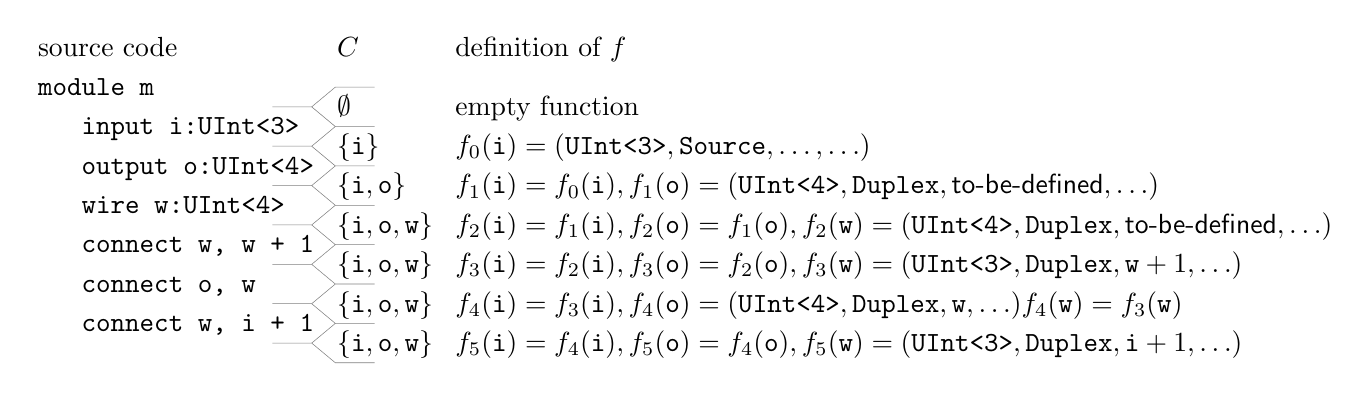
\begin{tikzpicture}
  \draw (0, 0.5) node[anchor=mid west]{source code}                  ++(3.8, 0)    node[anchor=mid west]{$C$}                                         ++(1.5,0) node[anchor=mid west]{definition of $f$};
  \draw (0, 0)   node[anchor=mid west]{\texttt{module m}}            ++(3.8,-0.25) node[anchor=mid west]{$\emptyset$}                                 ++(1.5,0) node[anchor=mid west]{empty function}
        (0,-0.5) node[anchor=mid west]{\texttt{~~~input i:UInt<3>}}  ++(3.8,-0.25) node[anchor=mid west]{$\{ \mathtt{i} \}$}                          ++(1.5,0) node[anchor=mid west]{$f_0(\mathtt{i}) = (\texttt{UInt<3>}, \mathtt{Source}, \ldots, \ldots)$}
        (0,-1.0) node[anchor=mid west]{\texttt{~~~output o:UInt<4>}} ++(3.8,-0.25) node[anchor=mid west]{$\{ \mathtt{i}, \mathtt{o} \}$}              ++(1.5,0) node[anchor=mid west]{$f_1(\mathtt{i}) = f_0(\mathtt{i}), f_1(\mathtt{o}) = (\texttt{UInt<4>}, \mathtt{Duplex}, \needtobedefined, \ldots)$}
        (0,-1.5) node[anchor=mid west]{\texttt{~~~wire w:UInt<4>}}   ++(3.8,-0.25) node[anchor=mid west]{$\{ \mathtt{i}, \mathtt{o}, \mathtt{w} \}$}  ++(1.5,0) node[anchor=mid west]{$f_2(\mathtt{i}) = f_1(\mathtt{i}), f_2(\mathtt{o}) = f_1(\mathtt{o}), f_2(\mathtt{w}) = (\texttt{UInt<4>}, \mathtt{Duplex}, \needtobedefined, \ldots)$}
        (0,-2.0) node[anchor=mid west]{\texttt{~~~connect w, w + 1}} ++(3.8,-0.25) node[anchor=mid west]{$\{ \mathtt{i}, \mathtt{o}, \mathtt{w} \}$}  ++(1.5,0) node[anchor=mid west]{$f_3(\mathtt{i}) = f_2(\mathtt{i}), f_3(\mathtt{o}) = f_2(\mathtt{o}), f_3(\mathtt{w}) = (\texttt{UInt<3>}, \mathtt{Duplex}, \mathtt{w} + 1, \ldots)$}
        (0,-2.5) node[anchor=mid west]{\texttt{~~~connect o, w}}     ++(3.8,-0.25) node[anchor=mid west]{$\{ \mathtt{i}, \mathtt{o}, \mathtt{w} \}$}  ++(1.5,0) node[anchor=mid west]{$f_4(\mathtt{i}) = f_3(\mathtt{i}), f_4(\mathtt{o}) = (\texttt{UInt<4>}, \mathtt{Duplex}, \mathtt{w}, \ldots) f_4(\mathtt{w}) = f_3(\mathtt{w})$}
        (0,-3.0) node[anchor=mid west]{\texttt{~~~connect w, i + 1}} ++(3.8,-0.25) node[anchor=mid west]{$\{ \mathtt{i}, \mathtt{o}, \mathtt{w} \}$}  ++(1.5,0) node[anchor=mid west]{$f_5(\mathtt{i}) = f_4(\mathtt{i}), f_5(\mathtt{o}) = f_4(\mathtt{o}), f_5(\mathtt{w}) = (\texttt{UInt<3>}, \mathtt{Duplex}, \mathtt{i} + 1, \ldots)$};

  \draw[very thin,gray] (3.9,0.03) -- ++(0.5,0) -- ++(-0.5,0)
        -- ++(-0.3,-0.25) -- ++(-0.5,0) -- ++(0.5,0) -- ++(0.3,-0.25) -- ++(0.5,0) -- ++(-0.5,0)
        -- ++(-0.3,-0.25) -- ++(-0.5,0) -- ++(0.5,0) -- ++(0.3,-0.25) -- ++(0.5,0) -- ++(-0.5,0)
        -- ++(-0.3,-0.25) -- ++(-0.5,0) -- ++(0.5,0) -- ++(0.3,-0.25) -- ++(0.5,0) -- ++(-0.5,0)
        -- ++(-0.3,-0.25) -- ++(-0.5,0) -- ++(0.5,0) -- ++(0.3,-0.25) -- ++(0.5,0) -- ++(-0.5,0)
        -- ++(-0.3,-0.25) -- ++(-0.5,0) -- ++(0.5,0) -- ++(0.3,-0.25) -- ++(0.5,0) -- ++(-0.5,0)
        -- ++(-0.3,-0.25) -- ++(-0.5,0) -- ++(0.5,0) -- ++(0.3,-0.25) -- ++(0.5,0) -- ++(-0.5,0)
        -- ++(-0.3,-0.25) -- ++(-0.5,0) -- ++(0.5,0) -- ++(0.3,-0.25) -- ++(0.5,0) -- ++(-0.5,0);
\end{tikzpicture}

\paragraph{Example of a bidirectional connection.}
The following code fragment illustrates how bidirectional connections are handled.

\noindent
\texttt{~~~input Bus\_in:\{data:UInt<32>, valid:UInt<1>, flip ack:UInt<1>\} \\
\mbox{}~~~wire internal\_Bus:\{data:UInt<32>, valid:UInt<1>, flip ack:UInt<1>\} \\
\mbox{}~~~connect internal\_Bus, Bus\_in}

leads to connections:
\begin{align*}
   f(\mathtt{Bus\_in}) & = (\{ \texttt{data:UInt<32>, valid:UInt<1>, flip ack:UInt<1>} \}, \mathtt{Source}, \\
                       & \phantom{{}={}}\ldots, \\
                       & \phantom{{}={}}\{ \texttt{data} := \mathord{\ldots}, \texttt{valid} := \mathord{\ldots}, \texttt{ack} := \texttt{internal\_Bus.ack} \}) \\
   f(\mathtt{internal\_Bus}) & = (\{ \texttt{data:UInt<32>, valid:UInt<1>, flip ack:UInt<1>} \}, \mathtt{Duplex}, \\
                       & \phantom{{}={}}\{ \mathtt{data} := \mathtt{Bus\_in.data}, \mathtt{valid} := \mathtt{Bus\_in.valid}, \mathtt{ack} := \mathord{\ldots} \}, \\
                       & \phantom{{}={}}\{ \mathtt{data} := \mathord{\ldots}, \mathtt{valid} := \mathord{\ldots}, \mathtt{ack} := \needtobedefined \})
\end{align*}

We see that a bidirectional connection needs to distinguish cases between adapting the first or the second expression.

\section{Semantic of a module}

Assume given a FIRRTL module $(\mathit{name}, \mathit{portlist}, \mathit{stmtlist})$.
Let $f: D \to \expressions(R) = \stmtsem(\mathit{name}, \linebreak[0] \portsem(\mathit{name}, \linebreak[0] \mathit{portlist}), \linebreak[0] \mathit{stmtlist})$ be its connection summary.
This operator is regarded as a transformation of an assignment $s: R \to \mathbb{V}$
to an assignment $f \circ s: D \to \mathbb{V}$
(where $\mathbb{V}$ is the range of concrete values that the variables in $R$ and $D$ can take, typically a subset of the integers).

Given a connection summary $f$ and an input assignment $s: R \to \mathbb{V}$ as above, we define the output assignment $f \circ s: D \to \mathbb{V}$ that results from applying $f$ to $s$ as:
$f \circ s(d) = f(d) \circ s$, i.e.\@ we evaluate the formal expression $f(d)$ by inserting the values from $s$ for concrete elements of $R$.

We also define an input extractor as follows: given an output assignment $s : D \to \mathbb{V}$ and a default input assignment $\mathit{dft} : R \to \mathbb{V}$,
we set $\extractinput{s}{\mathit{dft}} = s(r)$ if $r \in R \cap D$ and $\mathit{dft}(r)$ otherwise.

We then define the semantic of the module to be the least fixed point of $f$, in the sense:
given an input assignment $\mathit{is} : R \to \mathbb{V}$ (defined on $R$),
we take the output assignment $f \circ \mathit{is}$ as a starting point.
Then we repeatedly apply $f \circ \extractinput{\,\cdot\,}{\mathit{is}}$ to the output assignment, until we reach a fixed point
(or until it has become clear that no fixed point exists).
The fixed point output assignment is the semantic of the module.

\textbf{TODO:} Include registers and memories in this definition. \textbf{:END TODO}

\subsection{Example}

Continuing the above example,
let us take the input assignment $\mathit{is} : \{ \mathtt{w}, \mathtt{i} \} \to \mathbb{N}$ defined by $\mathit{is}(\mathtt{w}) = 3$ and $\mathit{is}(\mathtt{i}) = 1$.
The iteration works as follows:

\medskip

\noindent
\begin{tabular}{r@{${}:={}$}r|r@{${}\to{}$}l|l}
\multicolumn{2}{l|}{function} & \multicolumn{2}{l|}{type} & definition \\
$\mathit{is}_0$&$\mathit{is}\phantom{))}$ & $\{ \mathtt{w}, \mathtt{i} \}$&$\mathbb{N}$ & $\mathtt{w} \mapsto 3$, $\mathtt{i} \mapsto 1$ \\
$\mathit{os}_1$&$f_5 \circ \mathit{is}\phantom{))}$ & $\{ \mathtt{o}, \mathtt{w} \}$&$\mathbb{N}$ & $\mathtt{o} \mapsto \phantom{\mathit{os}}\llap{$\mathit{is}$}_0(\mathtt{w}) = 3$, $\mathtt{w} \mapsto \mathit{is}_0(\mathtt{i}) + 1 = 2$ \\
$\mathit{is}_1$&$\extractinput{f_5 \circ \mathit{is}}{\mathit{is}}\phantom{)}$ & $\{ \mathtt{w}, \mathtt{i} \}$&$\mathbb{N}$ & $\mathtt{w} \mapsto \mathit{os}_1(\mathtt{w}) = 2$, $ \mathtt{i} \mapsto \mathit{is}(\mathtt{i}) = 1$ \\
$\mathit{os}_2$&$f_5 \circ \extractinput{f_5 \circ \mathit{is}}{\mathit{is}}\phantom{)}$ & $\{ \mathtt{o}, \mathtt{w} \}$&$\mathbb{N}$ & $\mathtt{o} \mapsto \phantom{\mathit{os}}\llap{$\mathit{is}$}_1(\mathtt{w}) = 2$, $\mathtt{w} \mapsto \mathit{is}_1(\mathtt{i}) + 1 = 2$ \\
$\mathit{is}_2$&$\extractinput{f_5 \circ \extractinput{f_5 \circ \mathit{is}}{\mathit{is}}}{\mathit{is}}$ & $\{ \mathtt{w}, \mathtt{i} \}$&$\mathbb{N}$ & $\mathtt{w} \mapsto \mathit{os}_2(\mathtt{w}) = 2$, $ \mathtt{i} \mapsto \mathit{is}(\mathtt{i}) = 1$ \\
$\mathit{os}_3$&$f_5 \circ \extractinput{f_5 \circ \extractinput{f_5 \circ \mathit{is}}{\mathit{is}}}{\mathit{is}}$ & $\{ \mathtt{o}, \mathtt{w} \}$&$\mathbb{N}$ & $\mathtt{o} \mapsto \phantom{\mathit{os}}\llap{$\mathit{is}$}_2(\mathtt{w}) = 2$, $\mathtt{w} \mapsto \mathit{is}_2(\mathtt{i}) + 1 = 2$ \\
\end{tabular}

\medskip

We now see that $\mathit{os}_2 = \mathit{os}_3$, so the fixpoint has been reached.

If we would have used $f_4$ (with the malformed connection $f_4(\mathtt{w}) = \mathtt{w} + 1$), we would never reach a fixpoint because none exists.
As the program contains 3~connect statements, we should reach the fixpoint within at most 3~iterations,
so if it hasn't been reached after 3~iterations we know that it does not exist.

\end{document}
